\begin{frame}
    \frametitle{定義}

    根據 \citet*{Horn-Reinhart-Trebesch-21} 2.1節的定義:
    \begin{block}{Official Lending}
        \small
        We code China's official lending to developing and emerging countries, measured as \textbf{direct lending by the state and state-owned entities.}
        \dots \\
        When applying this definition to China, official creditors include \textbf{China's central government}, government agencies such as the
\textbf{Ministry of Commerce}, as well as lending by China's state-owned policy banks, in particular by \textbf{China Development Bank (CDB)} and
\textbf{China Export-Import Bank (Ex-Im)}. This definition also captures lending by China's state-owned commercial banks such as \textbf{Indus-
trial and Commercial Bank of China (ICBC)} or \textbf{Bank of China (BoC)} and supplier credits by state-owned enterprises, \dots
    \end{block}

\end{frame}

\begin{frame}
    \frametitle{中國在借貸市場上的活躍程度}
    \begin{figure}
        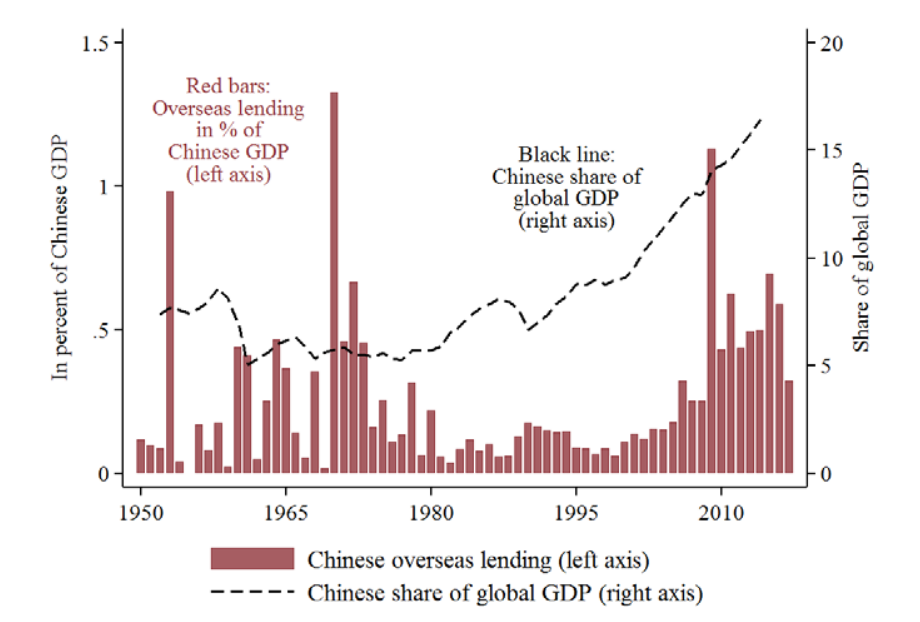
\includegraphics[width = \textwidth]{fig/fig4.png}
    \end{figure}
\end{frame}

\begin{frame}
    \begin{itemize}
        \item 1950s -- 1960s:援助共產國家
        \item 1980s -- 1990s:暫緩
        \item 2000s :GDP 成長,「走出去」策略
    \end{itemize}
\end{frame}

\begin{frame}
    \frametitle{援助國家比例}
    接受中國援助的開發中國家與興新國家比例
    \begin{figure}
        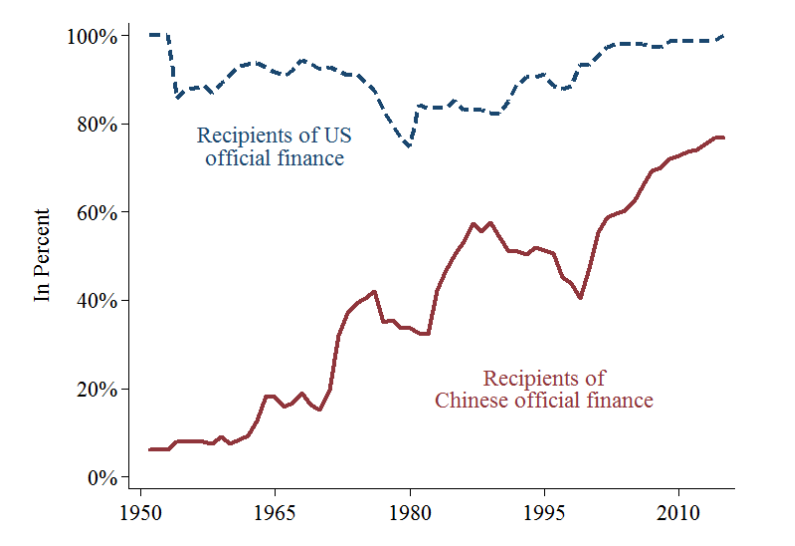
\includegraphics[height = 0.7\textheight]{fig/fig5.png}
    \end{figure}

\end{frame}

\begin{frame}
    \frametitle{對小國家的債務影響}

    \begin{itemize}
        \item 此資料庫優勢之一,是可以觀察接受中國援助的國家的債務程度。
        \item 有 30 幾個國家,對中國債務佔 GDP 比例超過 10\%
    \end{itemize}
    \begin{figure}
        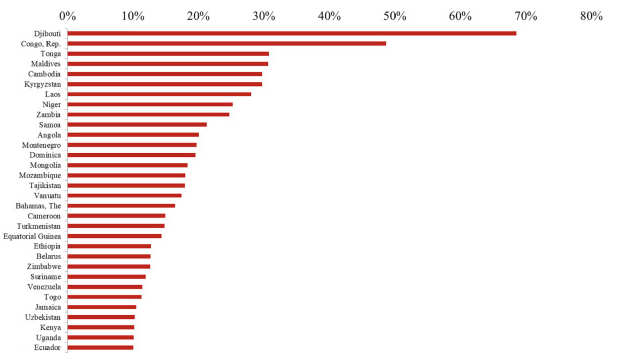
\includegraphics[height = 0.7\textheight]{fig/fig6.png}
    \end{figure}
\end{frame}

\begin{frame}
    \frametitle{有多少國家是重債窮國?}

    \begin{columns}
        \column{0.6\linewidth}
        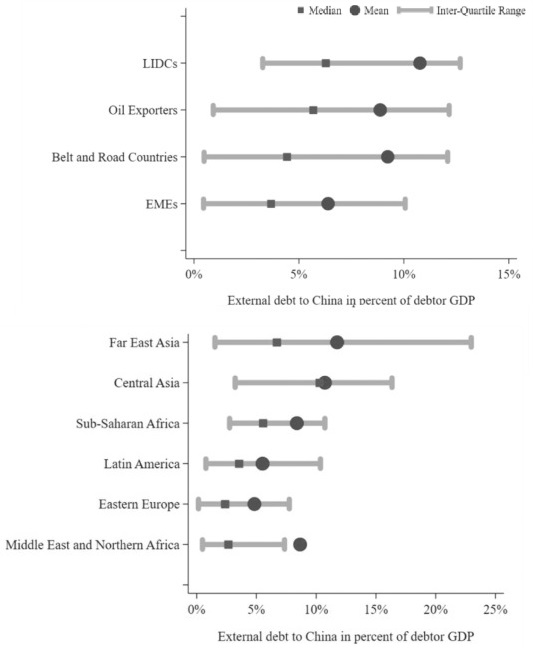
\includegraphics[height = 0.9\textheight]{fig/fig7.jpg}
        \column{0.4\linewidth}
        \begin{itemize}
            \item 低所得開發中國家 (LIDC) 平均 10.3\% 的 GDP為中國債務
            \item 一代一路國家 (BRI)中位數 4.4\%,但平均 9.2\%。表示有一些 BRI 的國家債務特別嚴重
            \item 債務最嚴重區域為東(南)亞國家。寮國、柬埔寨等。
        \end{itemize}
    \end{columns}

\end{frame}

\begin{frame}
    \frametitle{那相較於其他國際借貸者呢?}
        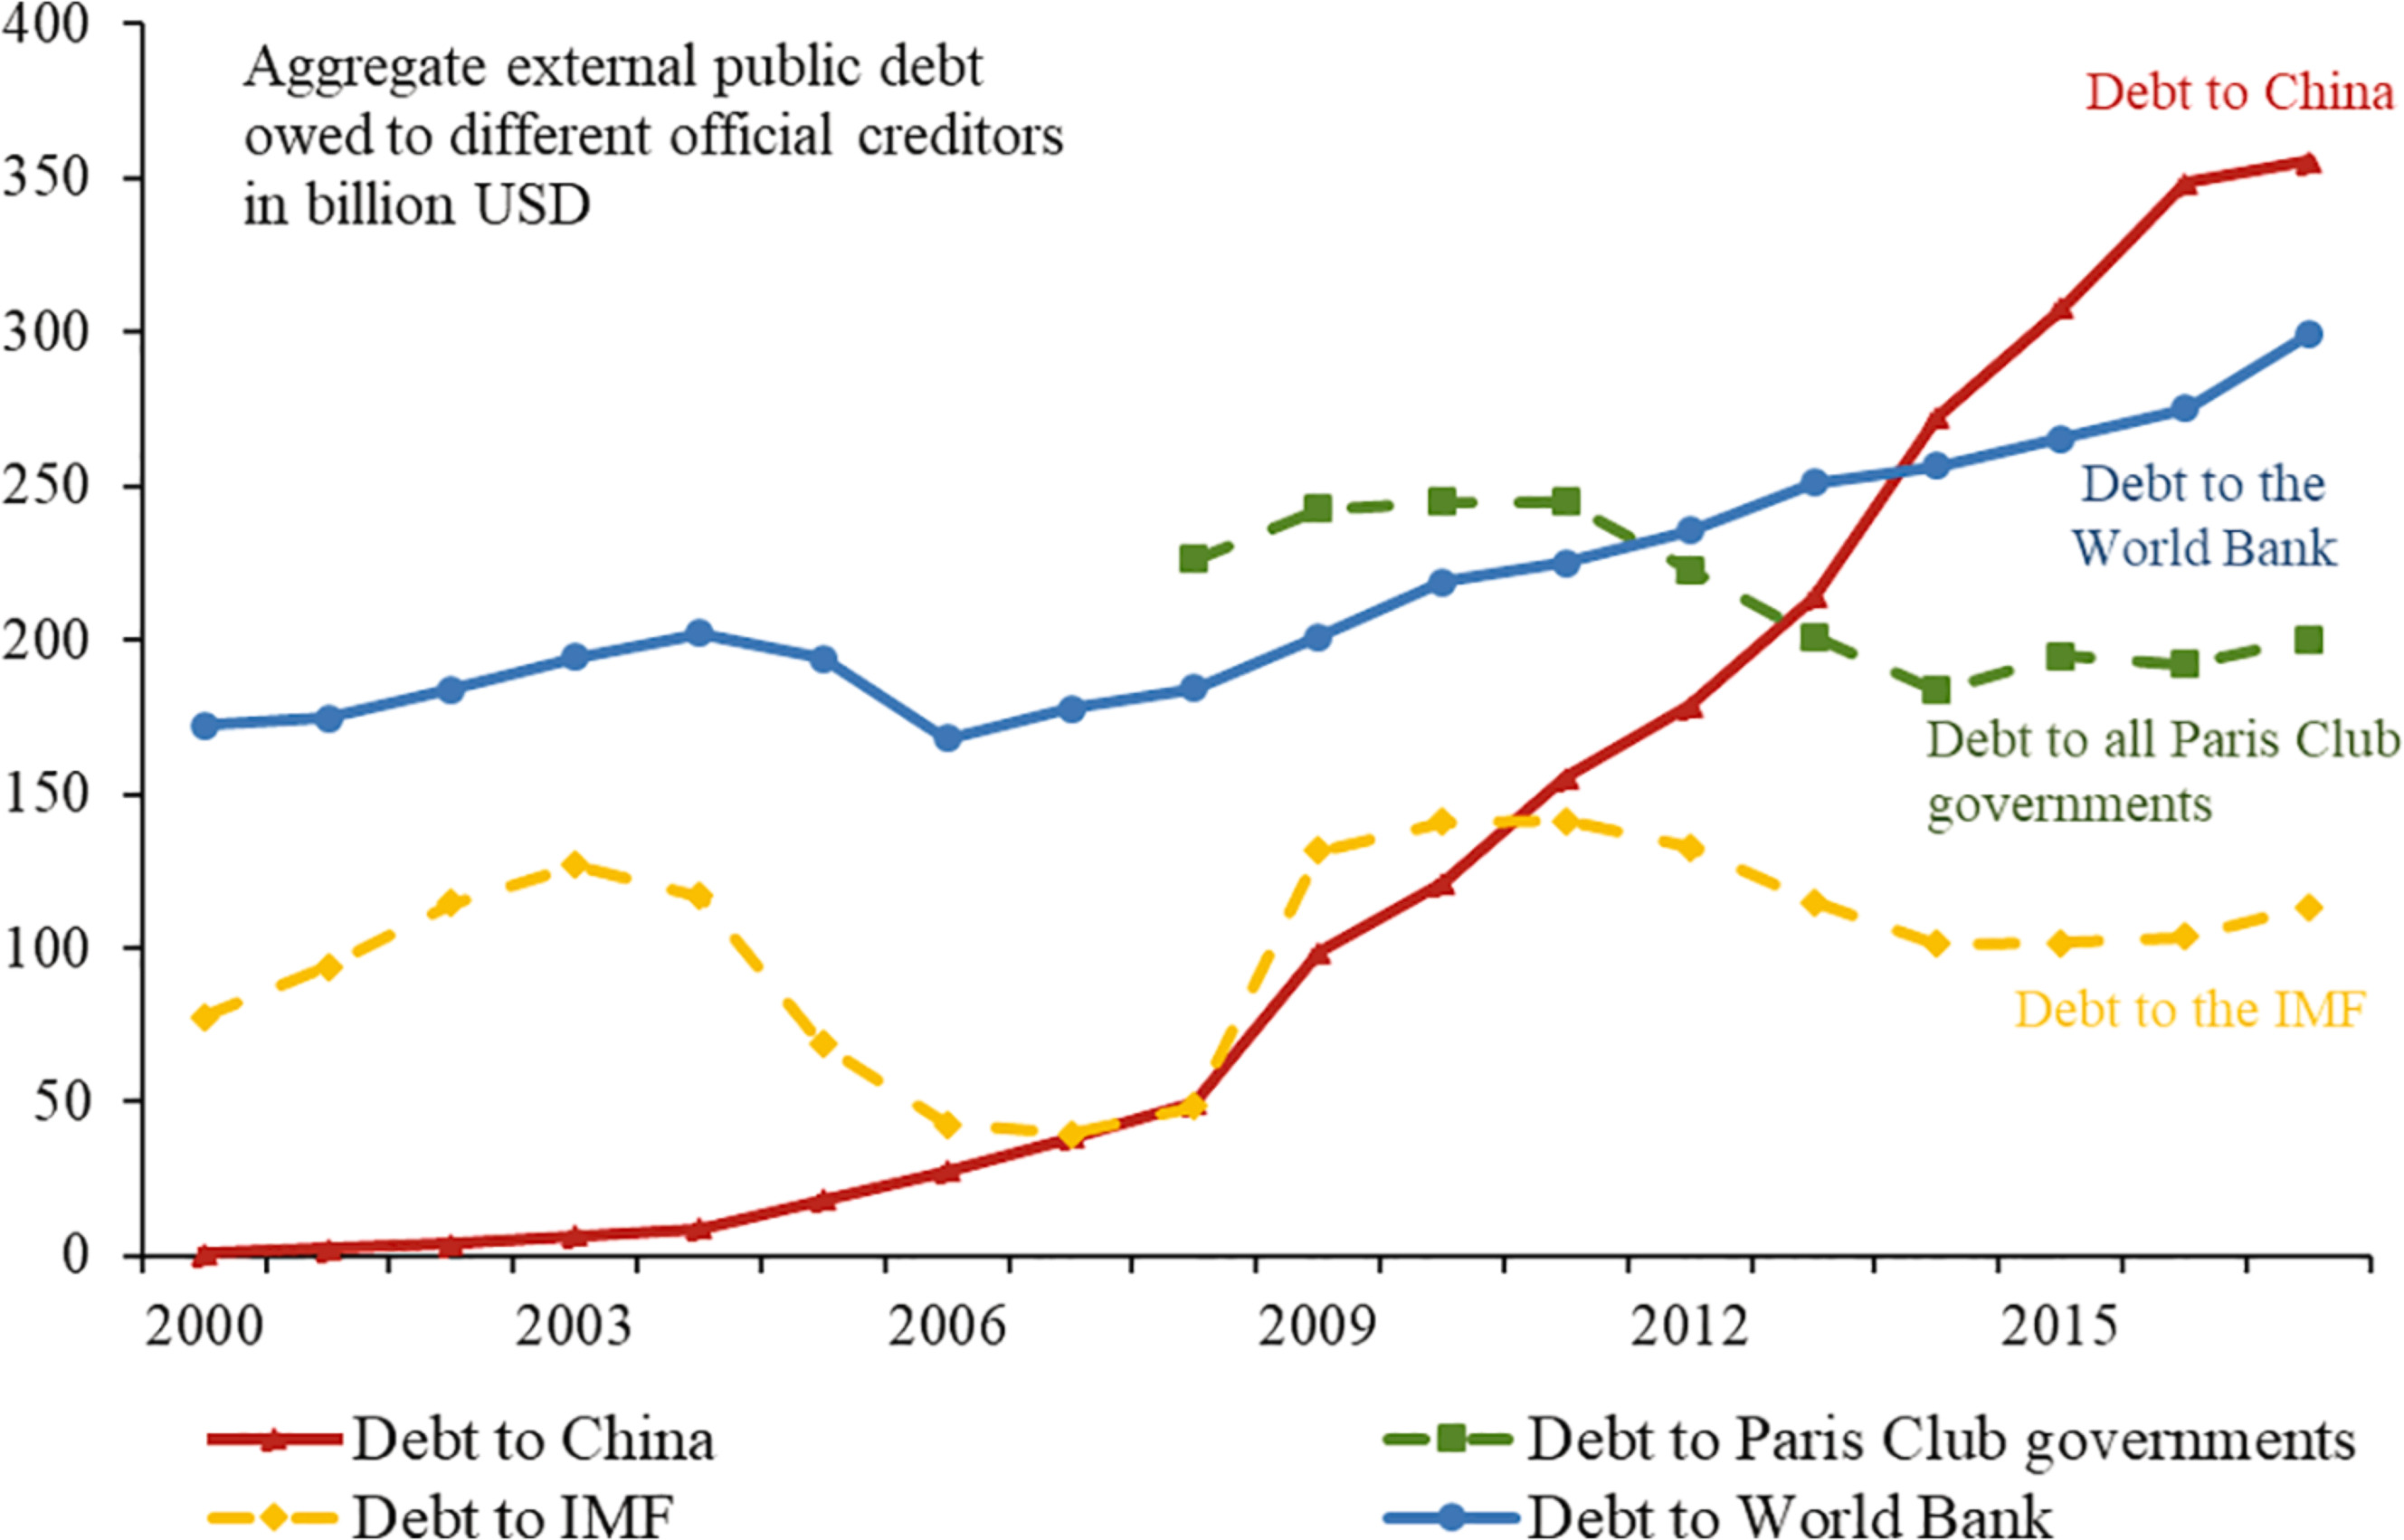
\includegraphics[width = \textwidth]{fig/fig9.jpg}
\end{frame}

\begin{frame}
    在 2017 年,各機構在開發中國家的總債權:
    \begin{itemize}
        \item 中國借出 3550 (億美金)
        \item 世界銀行借出 3000億
        \item 巴黎俱樂部所有會員國借出 2000億
    \end{itemize}

    \vfill
    中國已成為全球最大貸款者

\end{frame}

\begin{frame}
    \frametitle{債務內容}

    \begin{itemize}
        \item \citet*{Horn-Reinhart-Trebesch-21} 有個別貸款以及補助的資料
        \item 可以針對借貸合約內容進行統計
    \end{itemize}

    \vfill
    \begin{columns}
        \column[t]{0.5\textwidth}
        借出單位(貸方):
        \begin{itemize}
            \item 中國進出口銀行
            \item 中國開發銀行
            \item 合計超過 70\% 總借貸
        \end{itemize}
        借入單位(借方):
        \begin{itemize}
            \item 中央政府
            \item 國有企業
        \end{itemize}
        \column[t]{0.5\textwidth}
        利率:
        \begin{itemize}
            \item 比照商業借款(要付利息)
            \item 優惠貸款(concessional,無利息)
        \end{itemize}
        貨幣單位:
        \begin{itemize}
            \item 美金
            \item 人民幣
        \end{itemize}
    \end{columns}

\end{frame}

\begin{frame}

    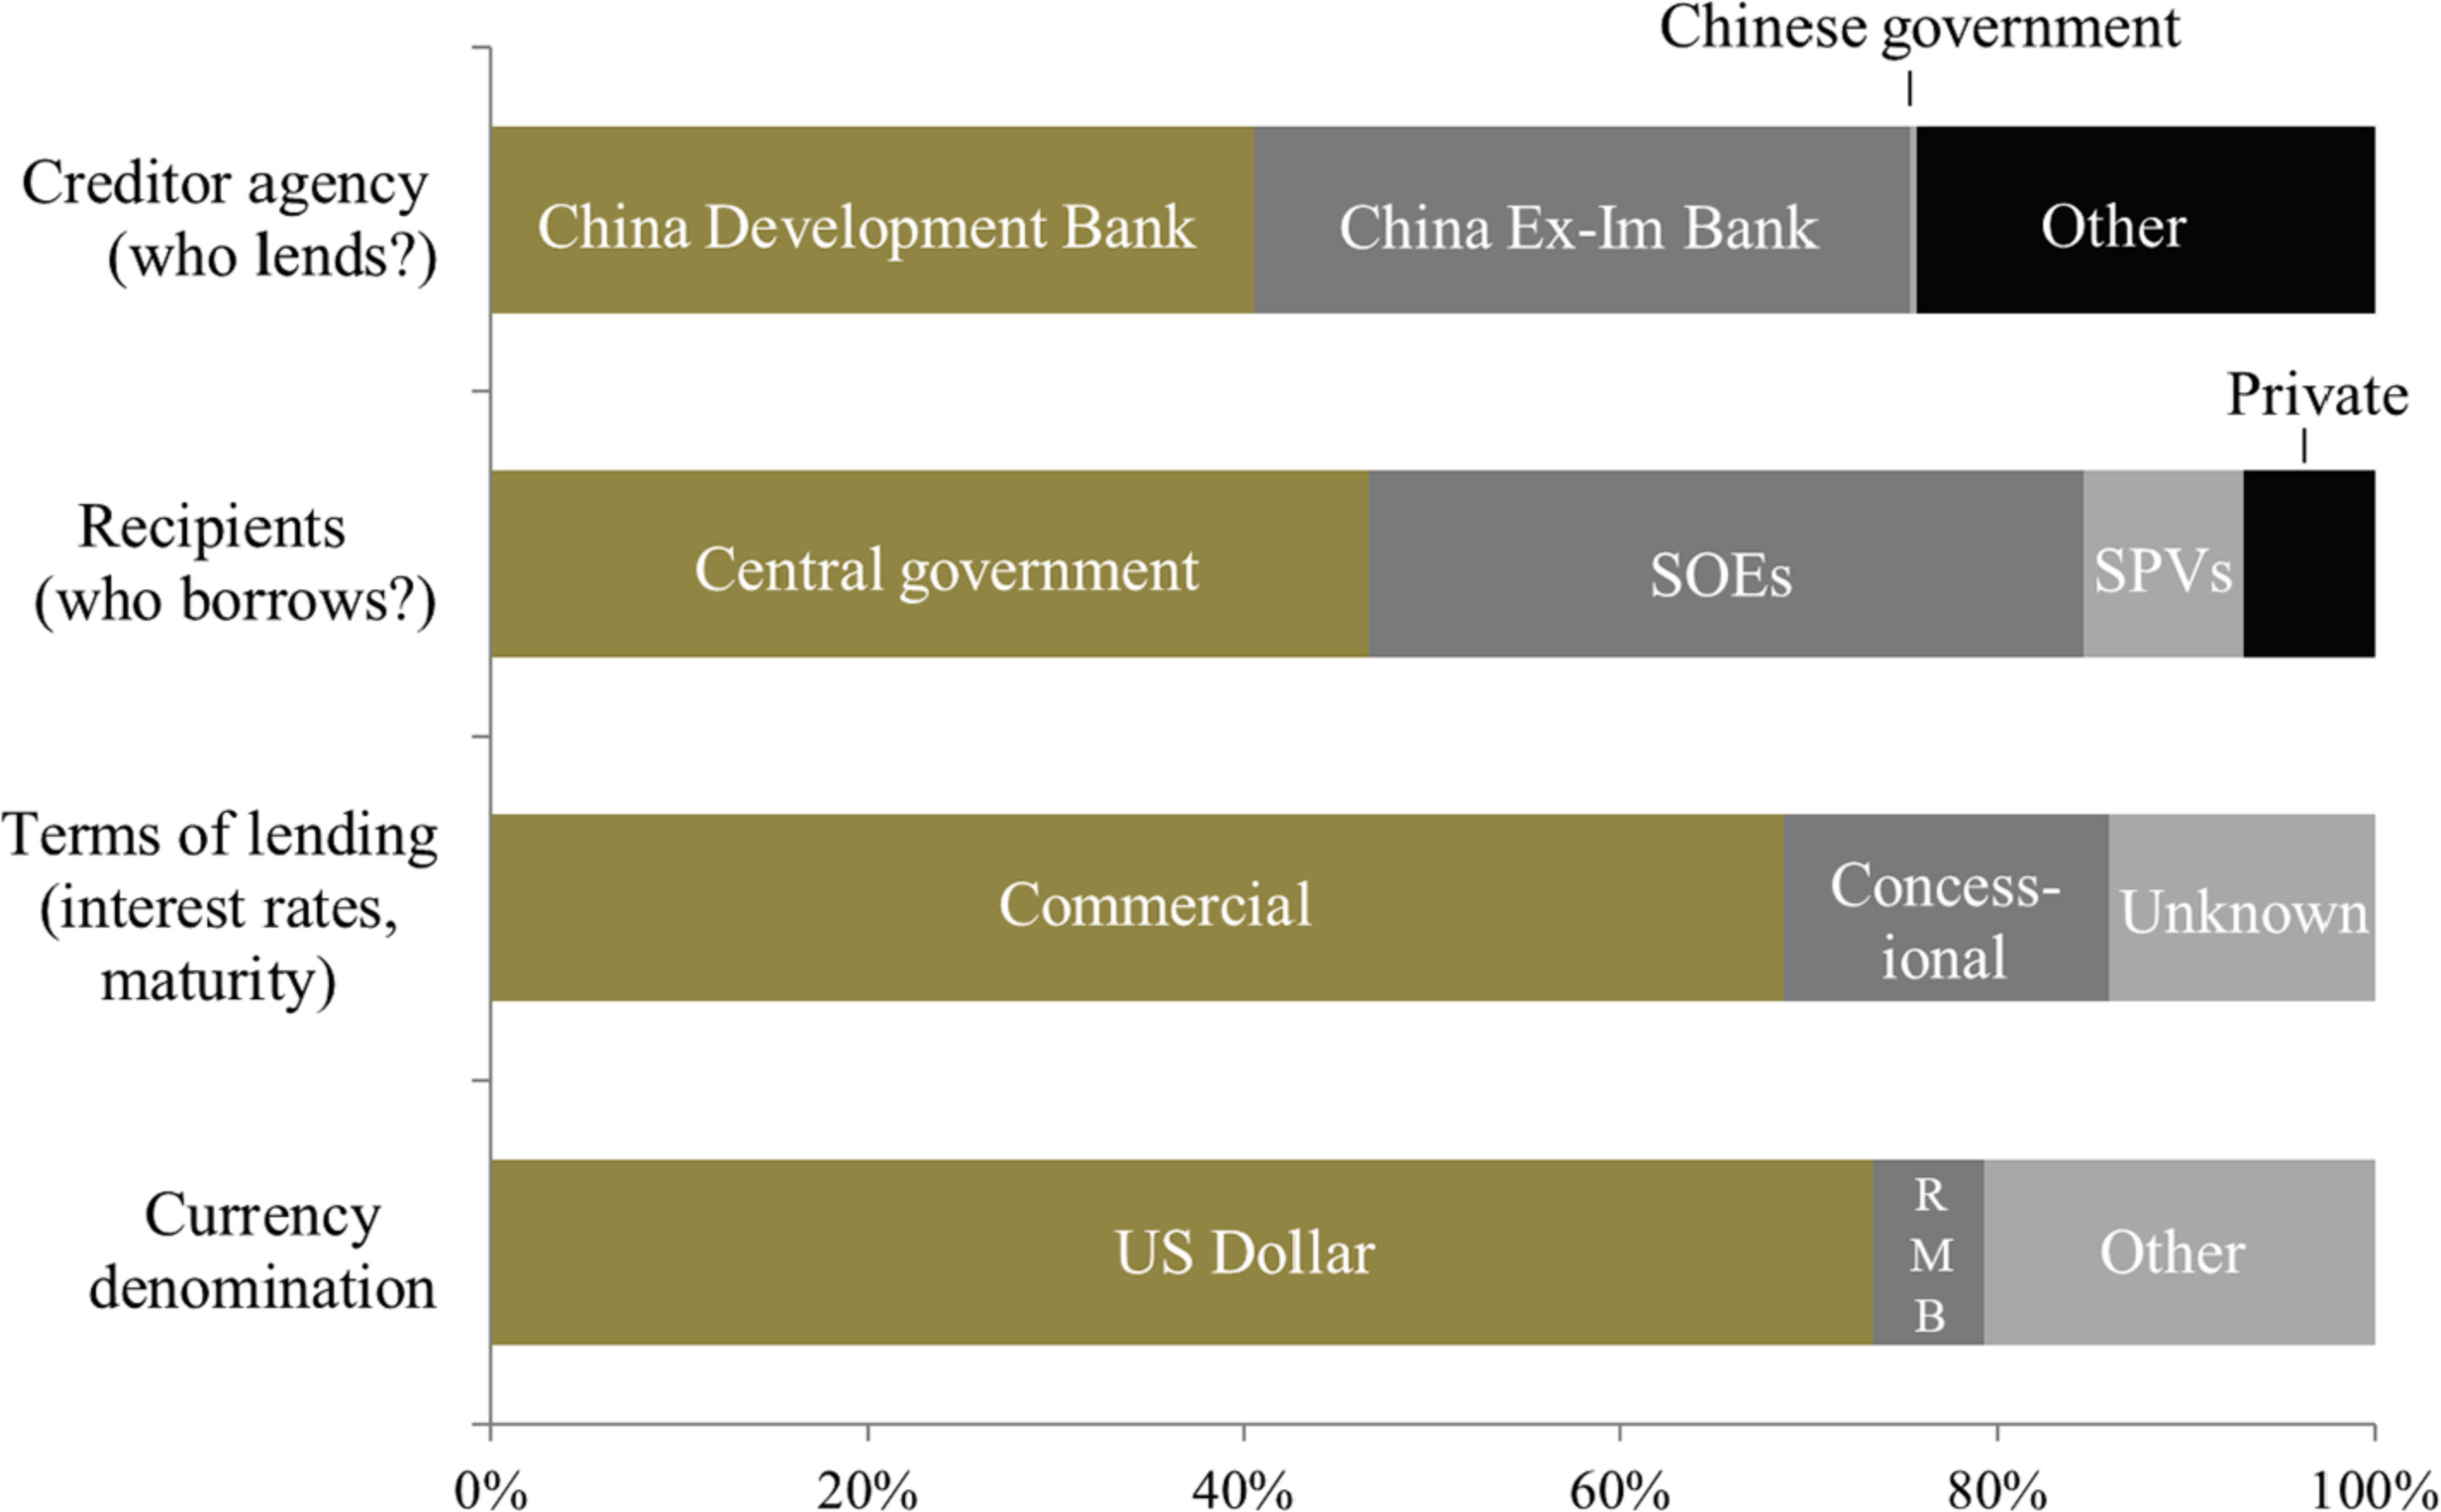
\includegraphics[width = \textwidth]{fig/fig10.jpg}

\end{frame}